% Chapter 1

\chapter{Introducción general} % Main chapter title

\label{Chapter1} % For referencing the chapter elsewhere, use \ref{Chapter1} 
\label{IntroGeneral}

%----------------------------------------------------------------------------------------

% Define some commands to keep the formatting separated from the content 
\newcommand{\keyword}[1]{\textbf{#1}}
\newcommand{\tabhead}[1]{\textbf{#1}}
\newcommand{\code}[1]{\texttt{#1}}
\newcommand{\file}[1]{\texttt{\bfseries#1}}
\newcommand{\option}[1]{\texttt{\itshape#1}}
\newcommand{\grados}{$^{\circ}$}

%----------------------------------------------------------------------------------------
%\section{Introducción}
En esta sección se da una introducción al protocolo CAN o \textit{Controller Area Network} \citep{web_cia_can} y al concepto de un servomotor. Se describe el proyecto SN-17, la motivación y alcance del trabajo y se resume el estado del arte de esta tecnología.

%----------------------------------------------------------------------------------------
\section{Controller area network}

CAN es un protocolo de comunicación desarrollado por la empresa Bosch \citep{can_basics_microchip} orientado originalmente a la industria automotriz. En el año 1991 Bosch publica la especificación CAN 2.0 y, en el año 1993, es adoptado internacionalmente bajo la norma ISO 11898 \citep{web_ISO_CAN}. Desde sus inicios el protocolo obtuvo gran popularidad y en la actualidad es utilizado en diversas industrias.

CAN se caracteriza por su robustez y bajos requerimientos de cableado. En su concepción fue pensado para proveer comunicaciones determinísticas en sistemas complejos. Este protocolo cuenta con \citep{UnderstandingCAN}:
\begin{itemize}
	\item Prioridad de mensajes y latencia máxima asegurada.
	\item Comunicaciones a varios dispositivos al mismo tiempo.	
	\item Bus multi-maestro.
	\item Detección de errores en nodos y mensajes.
	\item Protocolo asincrónico sin línea de clock.
\end{itemize}

Para realizar la transferencia de información CAN requiere únicamente 2 líneas de transmisión denominados CAN High (CAN H) y CAN Low (CAN L). Los mensajes CAN contienen un identificador que indica la prioridad del mensaje, así como a quien está dirigido. Usando esta información cada nodo de la red determina que acción debe realizar. En la figura \ref{fig:canBus} se presenta un esquema básico de una red CAN compuesta por 4 nodos.

\newpage

\begin{figure}[h!]
	\centering
	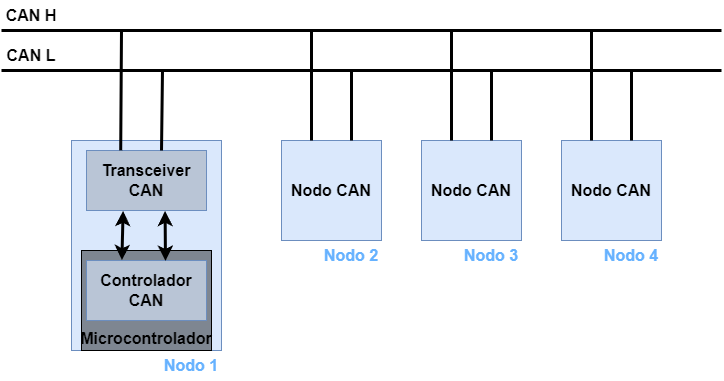
\includegraphics[scale=.5]{./Figures/CANBUS_Esquema.png}
	\caption{Esquema de red CAN.}
	\label{fig:canBus}
\end{figure}

%----------------------------------------------------------------------------------------

\section{Servomotores}

Un servomotor \citep{Industrial_Automation_Hands_On} es un tipo de motor eléctrico que tiene la capacidad de controlar la posición angular de su eje, así como la velocidad de rotación y el torque de salida. Esto se consigue con la utilización de un sistema de lazo cerrado de control que se retroalimenta con un sensor de posición angular llamado \textit{encoder}. En general, el tipo de bobinas del motor eléctrico no determina la condición de servomotor, sino que este cuente con las cualidades de control descriptas. En la figura \ref{fig:servomotor} \citep{web_partes_servomotor} se pueden observar las distintas partes que conforman un servomotor.

\begin{figure}[htbp]
	\centering
	\includegraphics[scale=0.8]{./Figures/servomotor.jpg}
	\caption{Partes de un servomotor\protect\footnotemark .}
	\label{fig:servomotor}
\end{figure}

\footnotetext{\url{https://www.logicbus.com.mx/blog/wp-content/uploads/2021/03/que-es-un-servomotor-773x400.jpg}} %Link a imagen de servomotor

%----------------------------------------------------------------------------------------

\section{Proyecto SN-17}

El proyecto SN-17 (Servo NEMA 17) es un sistema desarrollado como emprendimiento personal (A3 Engineering) que adapta motores eléctricos del tipo paso a paso o \textit{steppers} para funcionar como servomotores. El sistema SN-17 agrega un \textit{encoder} y un \textit{driver} al motor, los cuales generan un lazo cerrado, logrando así que el motor tenga las funcionalidades de un servomotor. En la figura \ref{fig:SN17} se puede observar una placa de control SN-17. Esta se coloca en la parte trasera del motor paso a paso.

\begin{figure}[htbp]
	\centering
	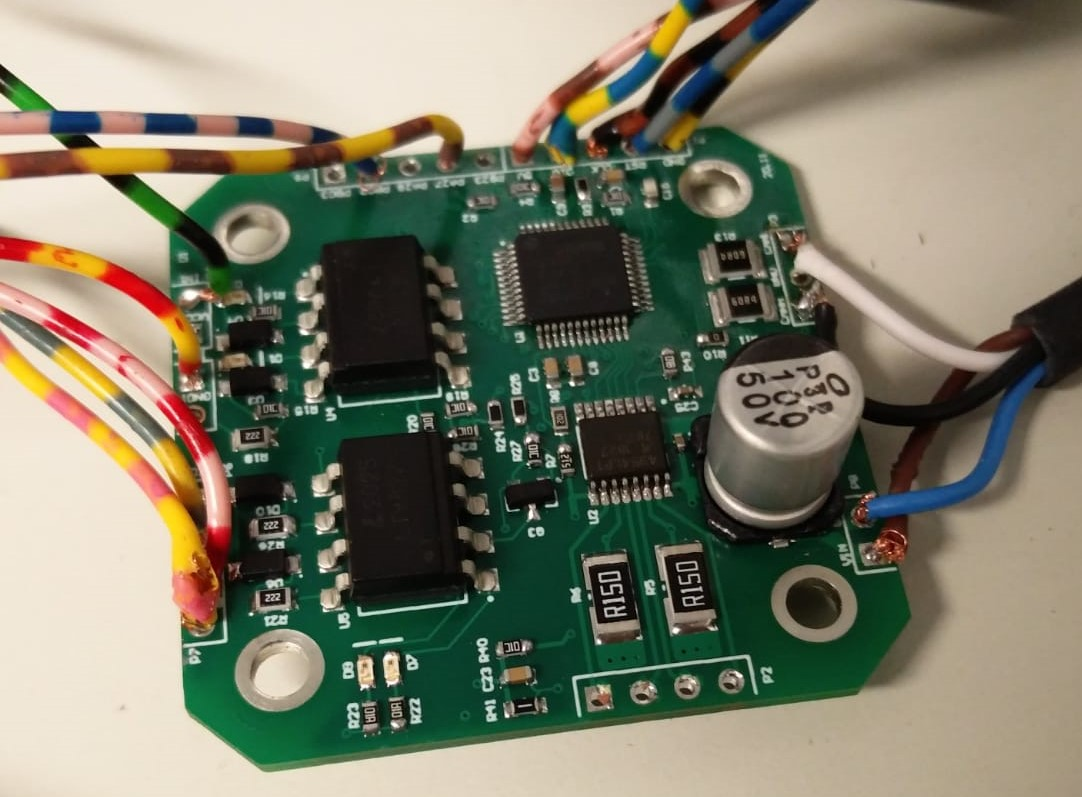
\includegraphics[scale=.3]{./Figures/SN17_5.jpeg}
	\caption{Plaqueta SN-17.}
	\label{fig:SN17}
\end{figure}

Además de generar las funcionalidades mencionadas, el sistema SN-17 utiliza señales discretas industriales que le permiten comunicarse con controladores de uso industrial (\textit{Programmable Logic Controllers} o PLCs).

Actualmente se está trabajando en implementar estos sistemas en la planta de la empresa Cambre ICyFSA \citep{web_cambre}, donde se están construyendo distintos dispositivos para aplicaciones industriales con estos motores. En la figura \ref{fig:aplicacionSN17} se puede observar un dibujo CAD de un actuador lineal con un sistema SN-17 implementado. Este funciona como un prensador en un proceso industrial.

\begin{figure}[h!]
	\centering
	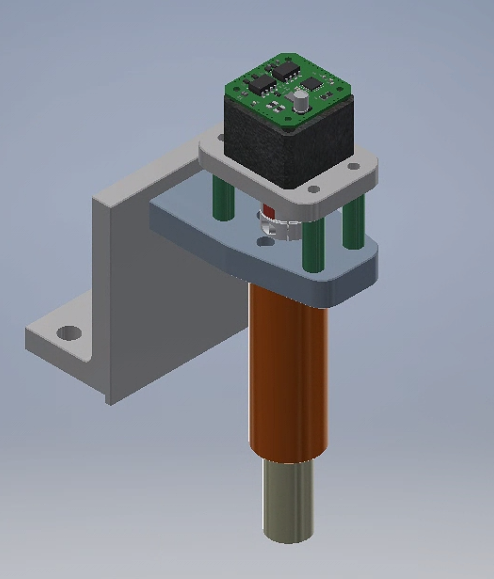
\includegraphics[width=0.6\linewidth ,height=0.25\textheight]{./Figures/Prensador-N17.PNG}
	\caption{Actuador lineal con SN-17.}
	\label{fig:aplicacionSN17}
\end{figure}

%----------------------------------------------------------------------------------------

\section{Motivación}
\label{motivacion}

En la actualidad el ámbito de actuadores industriales está principalmente dominado por aquellos de carácter neumático \citep{web_actuator_market}. Sin embargo, en los últimos años el uso de actuadores eléctricos ha empezado a ser más significativo debido a las mayores aptitudes de control que poseen y a sus menores costos operativos \citep{web_comparacion_actuadores}. En la tabla \ref{tab:comparacion_neumatico_electrico} se muestra una comparativa de ambos tipos de actuadores.

\begin{table}[htpb]
	\centering
	\caption[Comparación de actuadores neumáticos y eléctricos]{Comparación de actuadores neumáticos y eléctricos.}
	\begin{tabular}{c  c  c}    
		\toprule
		 	 & \textbf{Actuadores neumáticos}  & \textbf{Actuadores eléctricos}\\
		\midrule
		\textbf{Diseño} 			& Simple 		& Complejo  \\
		\textbf{Implementación} 	& Simple 		& Complejo \\			
		\textbf{Fuerza} 			& Según presión de aire	& Según reducción mecánica \\
		\textbf{Presición}			& Baja 	& Alta \\
		\textbf{Repetitibilidad}	& Baja 	& Alta \\
		\textbf{Eficiencia}			& Baja 	& Alta \\
		\textbf{Control de movimiento}	& Bajo 	& Alto \\
		\textbf{Mantenimiento}	& Alto 	& Bajo \\
		\bottomrule
		\hline
	\end{tabular}
	\label{tab:comparacion_neumatico_electrico}
\end{table}

Los actuadores eléctricos suelen emplear un servomotor en su interior que, junto con un mecanismo, generan el movimiento deseado con una precisión superior a los actuadores neumáticos. Aún así, este tipo de actuadores tienen como problema su elevado costo de adquisición y su dificultad de implementación, que limitan su uso. En este contexto, la organización A3 Engineering desarrolló el sistema SN-17 en un intento de disminuir los costos de los servomotores de aplicaciones pequeñas y, en un futuro, de los actuadores eléctricos.

La empresa Cambre ICyFSA instaló una serie de sistemas SN-17 en su planta productiva con resultados iniciales exitosos. Sin embargo, se limitó la implementación de más sistemas debido a su dificultad para reprogramarlos en momentos de necesidad. Esto se debe a que requieren de un cambio de \textit{firmware} para modificar su configuración y esto solo puede ser realizado por personal calificado. La motivación de este trabajo es brindar una interfaz para programación y monitoreo de una red de motores que pueda ser utilizada por personal no especializado.


%----------------------------------------------------------------------------------------

\section{Estado del arte}
\label{estado_del_arte}

Actualmente existe una extensa oferta de servomotores y motores paso a paso en el mercado. En general, lo que en el ámbito industrial se refiere a servomotores \citep{Industrial_Automation_Hands_On} son motores del tipo DC \textit{brushless} o AC de inducción (monofásicos y trifásicos). Estos tienen un precio significativamente mayor que los \textit{steppers} y suelen requerir de \textit{drivers} externos y, en caso de motores AC, variadores de frecuencia. En los casos en que se requiere alta potencia o alto rendimiento, estos servos son la opción indicada. Requieren de técnicos capacitados para su programación y ofrecen interfaces de usuario avanzadas. En general, representan soluciones de alto costo. Un motor AC de la empresa Panasonic \citep{web_servo_panasonic} junto con su \textit{driver} se presenta en la figura \ref{fig:ac-servo}. 


\begin{figure}[h!]
	\centering
	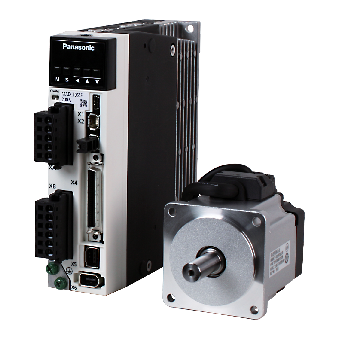
\includegraphics[scale=.65]{./Figures/ac-servo.png}
	\caption{Servomotor AC con \textit{driver}\protect\footnotemark.}
	\label{fig:ac-servo}
\end{figure}

\footnotetext{\url{https://assets.content.na.industrial.panasonic.com/public/styles/large/public/2019-11/A6_Servo_\%26_Drive_PHOTO_RGB_Panasonic_11-01-19.png?VersionId=Zy2t46MH7Tk5ce_Pw18lIwmTNWsf4YoK&itok=hJTUelmJ}} 


Por otro lado, en lo referido a motores \textit{steppers}, la oferta también es variada. Estos pueden adquirirse a precios muy accesibles y en distintos tamaños con lazo de control abierto. Requieren el uso de un \textit{driver} externo para su operación y su programación suele hacerse con software de terceros. Según la aplicación pueden requerir de conocimientos técnicos elevados. También existen variantes que agregan un \textit{encoder} de posición angular,  llamados \textit{closed loop steppers}. Estos solventan uno de los mayores problemas de estos motores relacionado con la pérdida de posición en caso de una perturbación, pero no permiten entregar torque constante. También requieren de \textit{drivers} externos y, según el fabricante, las interfaces de programación pueden ser complejas. Un ejemplo de un \textit{closed loop stepper} \citep{web_closed_loop_stepper} se presenta en la figura \ref{fig:closed-loop-stepper}, junto con su \textit{driver} correspondiente.

\begin{figure}[h!]
	\centering
	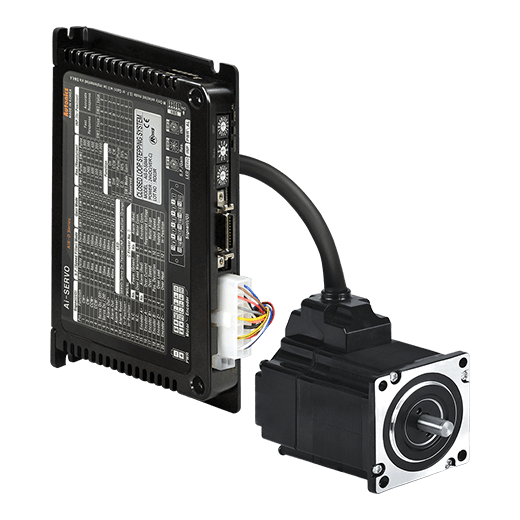
\includegraphics[scale=.35]{./Figures/closed_loop_stepper.png}
	\caption{\textit{Closed loop stepper} con \textit{driver}\protect\footnotemark .}
	\label{fig:closed-loop-stepper}
\end{figure}

\footnotetext{\url{https://www.autonics.com/web/2022/12/29/6/46/15/1032047e-1a41-4c24-aee4-966f2109fd40.png}} %Link a imagen de closed loop stepper

Finalmente, existen placas de control que, además de funcionar como un \textit{closed loop stepper}, tienen un \textit{driver} incorporado que permite controlar los motores de forma diferente, logrando entregar torque constante. El problema principal de estas soluciones es que suelen tener características de \textit{hobbista} y no son aptas para ámbitos industriales. También requieren de elevado conocimiento técnico para su programación debido a la falta de interfaces de usuario. En la figura \ref{fig:mechaduino} se puede ver un ejemplo de una de estas placas llamada \textit{Mechaduino} \citep{web_mechaduino}.

\begin{figure}[h!]
	\centering
	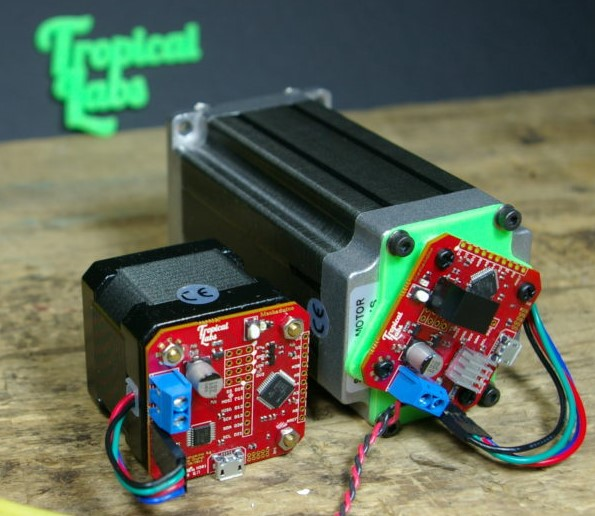
\includegraphics[scale=.6]{./Figures/mechaduino.jpg}
	\caption{Proyecto Mechaduino\protect\footnotemark .}
	\label{fig:mechaduino}
\end{figure}

\footnotetext{\url{https://tropical-labs.com/wp-content/uploads/2018/10/IMGP1300-1-1024x681.jpg}} %Link a imagen de mechaduino

En la Tabla \ref{tab:servos} se resume la información de los distintos tipos de motores mencionados.


\begin{table}[h!]
	\centering
	\caption[Estado del arte]{Resumen de características de servomotores.}
	\begin{tabular}{c c c c c}    
		\toprule
		\textbf{Motor} 	 & \textbf{Lazo de control}  & \textbf{\textit{Driver}} & \textbf{Programación} & \textbf{Precio (USD)} \\
		\midrule
		Servomotor & Cerrado & Externo & Compleja 	& >  1500 \\		
		\textit{Stepper open loop} & Abierto & Externo & Intermedia 	&  300\\
		\textit{Stepper closed loop} & Cerrado s/torque	& Externo & Intermedia 	&  400\\
		\textit{Mechaduino} & Cerrado	& Interno & Compleja 	&  200 \\
		SN-17 + interfaz	& Cerrado	& Interno & Simple 		&  300 \\
		\bottomrule
		\hline
	\end{tabular}
	\label{tab:servos}
\end{table}
%----------------------------------------------------------------------------------------

\section{Objetivos y alcance}

El objetivo de este trabajo es proporcionar una interfaz de usuario para el sistema SN-17 que permita que un operario no especializado pueda modificar los programas de los distintos motores conectados a través de una red CAN. La interfaz también debe poder emplearse para monitorear el estado de los motores conectados cuando están operativos. 

El proyecto incluye:

\begin{itemize}
	\item Una interfaz de usuario que permita configurar y supervisar los servomotores conectados.
	\item La construcción e implementación de la estructura de mensajes CAN.
	\item La configuración de la red CAN.
	\item El desarrollo y fabricación de una plaqueta con el sistema embebido.
	\item El desarrollo del firmware para este sistema y la adaptación del firmware del sistema SN-17.
\end{itemize}


